\chapter{Implementation}

The FFT algorithm has been implemented in C/C++, CUDA, OpenCL, DirectCompute and OpenGL on a GeForce GTX 670 and Radeon R7 260X graphics card and a Core i7 3770K 3.5GHz CPU.

\section{Algorithm}

The implementation can be broken down into a few steps, see figure \ref{fig:algorithm-overview} for an simplified overview. The algorithm setup is platform-dependant but some steps are common; get platform and device information, allocate device buffers and upload data to device.
\begin{figure}
	\centering
	\includestandalone[width=\textwidth]{figures/overview}
	\caption{Overview of the events in the algorithm.}
	\label{fig:algorithm-overview}
\end{figure}

The next step is to calculate the specific FFT arguments for a $N$-point sequence for each kernel. The most important difference between devices and platforms are local memory capacity and thread and block configuration. Threads per block was selected for the best performance. See table \ref{tab:threads-per-block} for details.
\begin{table}
	\centering
	\includestandalone[width=\textwidth]{tables/threadsperblock}
	\caption{Shared memory size, threads and block configuration per device.}
	\label{tab:threads-per-block}
\end{table}

The implementation of a $N$-point radix-2 FFT algorithm have $\log_2 N$ stages with $N/2$ butterfly operations per stage. A butterfly operation is an addition, a subtraction, followed by a multiplication by a twiddle factor, showed in figure \ref{fig:butterfly}.
\begin{figure}[h]
	\centering
	% FFT Butterfly
\tikzstyle{n}= [circle, fill, minimum size=4pt,inner sep=0pt, outer sep=0pt]
\tikzstyle{mul} = [circle,draw,inner sep=-1pt, minimum size=7pt]
\tikzstyle{sub} = [circle,draw,inner sep=-1pt, minimum size=7pt]
\tikzstyle{add} = [circle,draw,inner sep=-1pt, minimum size=7pt]

\begin{tikzpicture}[
	yscale=1.3,
	xscale=1.8,
	node distance=0.7cm,
	auto]
    
	\node[n, pin={[pin edge={latex'-,black}]left:$x(0)$}] (N-0-0) at (0,-0) {};
	\node[n, pin={[pin edge={latex'-,black}]left:$x(1)$}] (N-0-1) at (0,-1) {};
                            
	\node[add, name=N-1-0, pin={[pin edge={-latex',black},pin distance=1.175cm]right:$X(0)$}] at (1,-0) {${+}$};
	\node[sub, name=N-1-1, label={[label distance=-10pt]90:${-}$}] at (1,-1) {};
            
	\node[mul, right of=N-1-1, label={above right:\tiny $W^{k}_{N}$},
		pin={[pin edge={-latex',black}]right:$X(1)$}] (N-2-1) {${\times}$};       

	\path (N-0-0) edge[-latex'] (N-1-0);	
	\path (N-0-1) edge[-latex'] (N-1-1);
	\path (N-1-1) edge[-latex'] (N-2-1);
      
    % Connect nodes
    \foreach \src / \dst in {	0/0, 0/1, 1/0, 1/1}
       \path (N-0-\src.east) edge[-latex'] (N-1-\dst.west);
       
\end{tikzpicture}
	\caption{Butterfly operations}
	\label{fig:butterfly}
\end{figure}

The thread and block scheme was one butterfly per thread, so that a sequence of sixteen points require eight threads. Each platform was configured to a number of threads per block (see table \ref{tab:threads-per-block}) and any sequences twice as long as the threads per block configuration needed the algorithm to be split over several blocks. Example: if the threads per block limit is two, then four blocks would be needed for a sixteen point sequence.
\begin{figure}
	% FFT Butterfly
\tikzstyle{n}= [circle, fill, minimum size=4pt,inner sep=0pt, outer sep=0pt]
\tikzstyle{mul} = [circle,draw,inner sep=-1pt]

% Define two helper counters
\newcounter{x}\newcounter{y}
\begin{tikzpicture}[%
	yscale=0.6,
	xscale=1.15,
	node distance=0.25cm,
	auto]
    % The strategy is to create nodes with names: N-column-row
    % Input nodes are named N-0-0 ... N-0-15
    % Output nodes are named N-10-0 ... N-10-15

    % Draw inputs
    \foreach \y in {0,...,15}
        \node[n, pin={[pin edge={latex'-,black}]left:$x(\y)$}] (N-0-\y) at (0,-\y) {};
              
    % Draw outputs
    \foreach \y in {0,...,15}
        \node[n, pin={[pin edge={-latex',black}]right:$X(\y)$}] (N-11-\y) at (8,-\y) {};
              
   % draw connector nodes
    \foreach \y in {0,...,15}
        \foreach \x / \c in {1/1,2/3,3/4,4/6,5/7,6/9,7/10}
            \node[n, name=N-\c-\y] at (\x,-\y) {};
            
    % draw x nodes
    \foreach \y in {0,...,7}
        \foreach \x / \c  in {1/2}
            \node[mul, right of=N-\x-\y] (N-\c-\y) {};            
    \foreach \y in {8,...,15}
        \foreach \x / \c  in {1/2}
            \node[mul, right of=N-\x-\y] (N-\c-\y) {${\times}$};
    % 
    \foreach \y in {0,...,3}
        \foreach \x / \c  in {4/5}
            \node[mul, right of=N-\x-\y] (N-\c-\y) {};
    \foreach \y in {4,...,7}
        \foreach \x / \c  in {4/5}
            \node[mul, right of=N-\x-\y] (N-\c-\y) {${\times}$};
    \foreach \y in {8,...,11}
        \foreach \x / \c  in {4/5}
            \node[mul, right of=N-\x-\y] (N-\c-\y) {};
    \foreach \y in {12,...,15}
        \foreach \x / \c  in {4/5}
            \node[mul, right of=N-\x-\y] (N-\c-\y) {${\times}$};
    % 
    \foreach \y in {0,2,4,6,8,10,12,14}
        \foreach \x / \c  in {7/8}
            \node[mul, right of=N-\x-\y] (N-\c-\y) {};
    \foreach \y in {1,3,5,7,9,11,13,15}
        \foreach \x / \c  in {7/8}
            \node[mul, right of=N-\x-\y] (N-\c-\y) {${\times}$};    

    % horizontal connections
    % Note the use of simple counter arithmetics to get correct
    % indexes.
    \foreach \y in {0,...,15}
    {
		\foreach \x in {0,1,3,4,7}
		{
			\setcounter{x}{\x}\stepcounter{x}
			\path (N-\x-\y) edge[-] (N-\arabic{x}-\y);
		}
	}
       
    % Draw the W_16 coefficients
    \setcounter{y}{0}
    \foreach \i in {0,...,7}
    {
	   	\path (N-2-\arabic{y}) edge[-] node {} (N-3-\arabic{y});
	    \stepcounter{y}
    }
    \foreach \i in {0,...,7}
    {
    	\path (N-2-\arabic{y}) edge[-] node {\tiny $W^{\i}_{16}$} (N-3-\arabic{y});
        \stepcounter{y}
    }
    
    % Draw the W_8 coefficients
    \setcounter{y}{0}
    \foreach \tmp in {0,1}
	{
    	\foreach \i in {0,...,3}
    	{
        	\path (N-5-\arabic{y}) edge[-] node {} (N-6-\arabic{y});
        	\addtocounter{y}{1}
    	}
    	\foreach \i in {0,...,3}
    	{
        	\path (N-5-\arabic{y}) edge[-] node {\tiny $W^{\i}_{8}$} (N-6-\arabic{y});
        	\addtocounter{y}{1}
    	}
    }

    % Draw the W_4 coefficients
    \setcounter{y}{0}
	\foreach \tmp in {0,...,3}
	{    
		\foreach \i in {0,1}
		{
			\path (N-8-\arabic{y}) edge[-] node {} (N-9-\arabic{y});
			\stepcounter{y}
			\path (N-8-\arabic{y}) edge[-] node {\tiny $W^{\i}_{4}$} (N-9-\arabic{y});
			\stepcounter{y}
		}
    }
    
    % Connect nodes
    \foreach \sourcey / \desty in {	0/8,	1/9,	2/10,	3/11,
									4/12,	5/13,	6/14,	7/15,
									8/0,	9/1,	10/2,	11/3,
									12/4,	13/5,	14/6,	15/7}
       \path (N-0-\sourcey.east) edge[-] (N-1-\desty.west);
    \foreach \sourcey / \desty in {	0/4,	1/5,	2/6,	3/7,
									4/0,	5/1,	6/2,	7/3,
									8/12,	9/13,	10/14,	11/15,
									12/8,	13/9,	14/10,	15/11}
        \path (N-3-\sourcey.east) edge[-] (N-4-\desty.west);
    \foreach \sourcey / \desty in {	0/0,	1/2,	2/0,	3/2,
    								0/1,	1/3,	2/1,	3/3,
                                   	4/4,	5/6,	6/4,	7/6,
                                   	4/5,	5/7,	6/5,	7/7,
                                   	8/8,	9/10,	10/8,	11/10,
									8/9,	9/11,	10/9,	11/11,
									12/12,	13/14,	14/12,	15/14,
									12/13,	13/15,	14/13,	15/15}
	{
        \path (N-6-\sourcey.east) edge[-] (N-7-\desty.west);
        \path (N-9-\sourcey.east) edge[-] (N-10-\desty.west);
    }
    % Nodes are in bit-reverse order
    \foreach \sourcey / \desty in {	0/0,1/8,2/4,3/12,4/2,5/10,6,7/14,8/1,9,10/5,11/13,12/3,13/11,14/7,15/15}
	{
        \path (N-10-\sourcey.east) edge[-] (N-11-\desty.west);
    }
    
    % Add region boxes
	% Partial stage
	\def \lastNode {10}
	\node[draw,dashed,fit=(N-6-0) (N-\lastNode-3)] {};
	\node[draw,dashed,fit=(N-6-4) (N-\lastNode-7)] {};
	\node[draw,dashed,fit=(N-6-8) (N-\lastNode-11)] {};
	\node[draw,dashed,fit=(N-6-12) (N-\lastNode-15)] {};	
    % Complete stage
	\node[draw,densely dotted,fit=(N-0-0) (N-2-15),label=above:{stage 1}] {};
	\node[draw,densely dotted,fit=(N-3-0) (N-5-15),label=above:{stage 2}] {};
	\node[draw,fit=(N-6-0) (N-8-15),opacity=0,label=above:{stage 3},name=Stage-3] {};
	\node[draw,fit=(N-9-0) (N-\lastNode-15),opacity=0,label=above:{stage 4},name=Stage-4] {};
	\node[draw,fit=(N-11-0) (N-11-15),opacity=0,label=above:{output}] {};
	\node[draw,densely dotted,fit=(Stage-3) (Stage-4)] {};
	\node[draw,fit=(N-\lastNode-0) (N-11-15)] {};
\end{tikzpicture}
	\caption{Example flow graph of a sixteen-point FFT using (stage 1 and 2) Cooley-Tukey algorithm and (stage 3 and 4) constant geometry algorithm. The solid box is the bit-reverse order output. Dotted boxes are seperate kernel launches, dashed boxes are data transfered to local memory before computing the remaining stages.}
	\label{fig:flowgraph-16}
\end{figure}

Thread synchronization is only available within a block. When the sequence or partial sequence fitted within a block all data was transfered to local memory before completing the last stages. If the sequence was larger and required more then one block the synchronization was handled by launching several kernels executed in sequence. The kernel launched for block wide synchronization is called the global kernel and the kernel for thread synchronization within a block is called the local kernel. The global kernel had an implementation of the Cooley-Tukey FFT algorithm and the local kernel had constant geometry (same indexing for every stage). The last stage outputs from shared memory to the bit reversed index of the complete sequence. See figure \ref{fig:flowgraph-16} where the sequence length is sixteen and the thread per block is set to two.

The indexing for the global kernel was calculated from the thread id and block id (threadIdx.x and blockIdx.x in CUDA) as seen in figure \ref{fig:code-global-index}. Input and output is done on the same index.
\begin{figure}
	\centering
	\lstset{language=C++}
	\begin{framed}
	\begin{lstlisting}
int tid     = blockIdx.x * blockDim.x + threadIdx.x,
    io_low  = tid + (tid & (0xFFFFFFFF << stages_left)),
    io_high = index1 + (N >> 1);
	\end{lstlisting}
	\end{framed}
	\caption{ CUDA example code showing index calculation for each stage in the global kernel, N is the total number of points. }
	\label{fig:code-global-index}
\end{figure}

Index calculation for the local kernel is done once for all stages, see figure \ref{fig:code-local-index}. These indexes are seperate from the indexing in the global memory. The global memory offset depends on threads per block (blockDim.x in CUDA) and block id.
\begin{figure}
	\centering
	\lstset{language=C++}
	\begin{framed}
	\begin{lstlisting}
int n_per_block = N / gridDim.x.
    in_low      = threadId.x.
    in_high     = threadId.x + (n_per_block >> 1).
    out_low     = threadId.x << 1.
    out_high    = out1 + 1;
	\end{lstlisting}
	\end{framed}
	\caption{ CUDA example code showing index calculation for points in shared memory for the CUDA local kernel. }
	\label{fig:code-local-index}
\end{figure}

The last operation after the last stage is to perform the bit-reverse indexing operation, this is done when writing from shared to global memory. The implementation of bit reversing is available as a single instruction on some platforms, if not available figure \ref{fig:code-bit-reverse} shows the code used. The bit reversed value had to be right shifted the number of zeroes leading the number in a 32-bit int. Example of the bit-reverse index operation: index 8 of a 16 point sequence is bit-reversed to 1, in bit-representation (binary) its 1000 to 0001. Index 8 of a 32 point sequence is bit-reversed to 2, correspons to 01000 to 00010. Figure \ref{fig:flowgraph-16} show the complete bit-reverse operation of all point in the last step after the last stage.

\begin{figure}[h]
	\centering
	\lstset{language=C++}
	\begin{framed}
	\begin{lstlisting}
x = (((x & 0xaaaaaaaa) >> 1) | ((x & 0x55555555) << 1));
x = (((x & 0xcccccccc) >> 2) | ((x & 0x33333333) << 2));
x = (((x & 0xf0f0f0f0) >> 4) | ((x & 0x0f0f0f0f) << 4));
x = (((x & 0xff00ff00) >> 8) | ((x & 0x00ff00ff) << 8));
return((x >> 16) | (x << 16));
	\end{lstlisting}
	\end{framed}
	\caption{ Kernel code producing a bit reversed unsigned integer where x is the input. }
	\label{fig:code-bit-reverse}
\end{figure}

The FFT algorithm for two dimensional sequences, such as images, is first a transform of each row (each row as a seperate sequence) and then a transform of each column. This GPU implementation does the first rowwise transformation and then transposes the whole image and repeat these to operations. An example is shown in figure \ref{fig:twodimentransform}.
\begin{figure}
	\centering
	\subfloat[Original image\label{image-1:lena}]{
		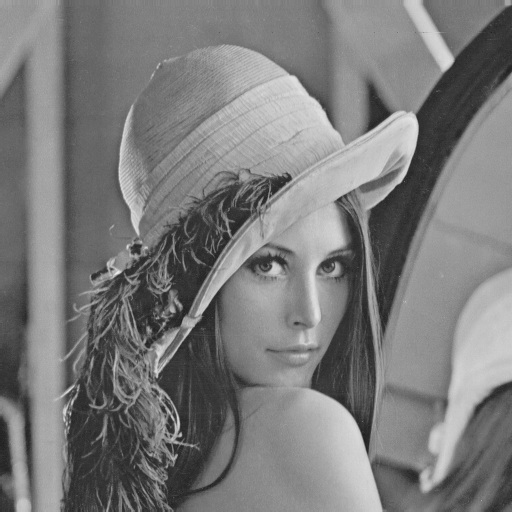
\includegraphics[keepaspectratio=true, scale=0.33]{images/lena.jpg}{}
    }
    \hfill
    \subfloat[Magnitude representation\label{image-2:lena}]{
		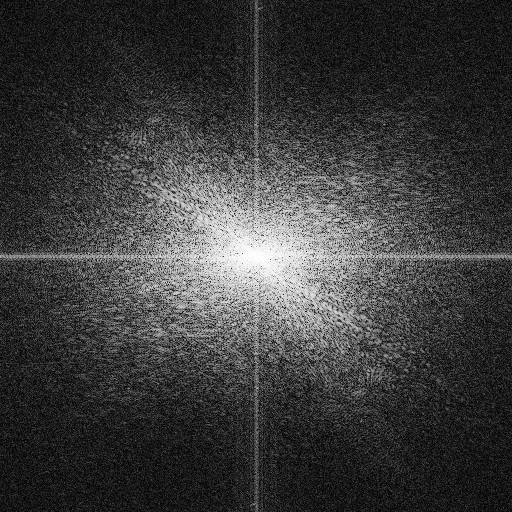
\includegraphics[keepaspectratio=true, scale=0.33]{images/lena_transformed.jpg}{}
    }
	\caption{Original image to the left. The image to the right is a quadrant shifted magnitude visualization of the original image. }
    \label{fig:twodimentransform}
\end{figure}